\documentclass{beamer}
%\usetheme{Ilmenau}
%\usecolortheme{beaver}

\usepackage[slovak,american]{babel}
\usepackage[utf8]{inputenc}
\usepackage{graphicx}
\usepackage{adjustbox}
\usepackage{xcolor}
\usepackage{mathrsfs}
 
 \newsavebox\MBox
\newcommand\Cline[2][red]{{\sbox\MBox{$#2$}%
  \rlap{\usebox\MBox}\color{#1}\rule[-2.2\dp\MBox]{\wd\MBox}{1pt}}}

%\usefonttheme{serif}

%\definecolor{UKOrange}{HTML}{ef9424} %
\definecolor{UKOrange}{HTML}{7a2c18} %
\definecolor{UKBrown}{HTML}{a96d5e} %
\definecolor{UKLight}{HTML}{d8b6ab} %
\definecolor{UKDark}{HTML}{7a4f44}
\definecolor{UKDarker}{HTML}{4d312b} 
\definecolor{UKDarkest}{HTML}{2e1e1a}
\definecolor{UKRed}{HTML}{bf1f1c}

\setbeamertemplate{footline}[frame number]{}
\setbeamertemplate{navigation symbols}{}

%\usecolortheme{beaver}
\setbeamertemplate{itemize item}[square]
\setbeamercolor{itemize item}{fg = UKBrown}
\setbeamercolor{itemize subitem}{fg = UKLight}
\setbeamercolor{enumerate item}{fg = UKDark}

\setbeamercolor{footnote}{fg=UKLight}
\setbeamercolor{footnote mark}{fg=UKLight}
\setbeamerfont{footnote}{size=\tiny}
\renewcommand\footnoterule{}

\usetheme{default}
\beamertemplatenavigationsymbolsempty
\setbeamercolor{title}{fg=white, bg=UKBrown}
\setbeamercolor{frametitle}{fg=white, bg=UKBrown}
\setbeamercolor{block title}{bg=UKBrown, fg= white}
\setbeamercolor{block body}{bg =UKLight, fg = UKDarkest}

\setbeamercolor{block title alerted}{bg=UKOrange, fg= white}
\setbeamercolor{block body alerted}{bg =UKLight, fg = UKDarkest}


%\setbeamercolor{section in toc}{fg = UKBrown}
%\setbeamercolor{section in toc}{fg = UKDarkest}

% odstrani gulicky
\renewcommand*{\slideentry}[6]{}

\useoutertheme[subsection=false]{miniframes}
\AtBeginSection[]{\subsection{}}

\setbeamercolor{below lower separation line head}{bg=UKDark}
\addtobeamertemplate{headline}{}{%
  \begin{beamercolorbox}[colsep=0.5pt]{below lower separation line head}
  \end{beamercolorbox}
}
%\setbeamercolor*{mini frame}{fg=white,bg=UKRosy}
\setbeamercolor{section in head/foot}{fg=UKLight, bg=UKDark}

\usepackage{etoolbox}
\makeatletter
\preto{\@verbatim}{\topsep=0pt \partopsep=0pt }
\makeatother

%\setbeamertemplate{itemize/enumerate body begin}{\normalsize}
%\setbeamertemplate{itemize/enumerate subbody begin}{\normalsize}




%\newcommand{\codeblock}[2]{ \begin{block}{#1} \begin{verbatim}#2\end{verbatim}\end{block}}

%\defbeamertemplate*{title page}{customized}[1][]
%{
%  \begin{centering}
%    \begin{beamercolorbox}[sep=8pt,center]{title}
%      \usebeamerfont{title}\inserttitle
%    \end{beamercolorbox}
%  \end{centering}
%  \bigskip
%
%\begin{columns}[onlytextwidth,T]
%
%
%  \column{27mm}
%  \includegraphics[width=27mm]{images/logoFMFI.png}
%  
%  \column{\dimexpr\linewidth-54mm-6mm}
%  \centering
%  \vspace{5mm}  
%  \usebeamerfont{author}\insertauthor\par
%  \vspace{5mm}
%  \usebeamerfont{institute}\insertinstitute\par
%
%  \column{27mm}
%  \includegraphics[width=27mm]{images/logoUK.png}  
%\end{columns}
%\centering
%\vspace{7mm}
%  \usebeamerfont{date}\insertdate\par
%}

\DeclareMathOperator*{\argmin}{arg\,min}
\newcommand{\e}[1]{$\cdot 10^{#1}$}

%\newcommand{\codeblock}[2]{ \begin{block}{#1} \begin{verbatim}#2\end{verbatim}\end{block}}



\title[11. cvičenie]{Advanced Image Processing - Image Transformations}
\author[Kocur]{Ing. Viktor Kocur \\{\small viktor.kocur@fmph.uniba.sk}}
\institute{DAI FMFI UK}
\date{4.12.2019}

\begin{document}
\selectlanguage{american}

\begin{frame}

  \titlepage

\end{frame}

\section{Image Resizing}


\begin{frame}
\frametitle{Information in images}
\centering
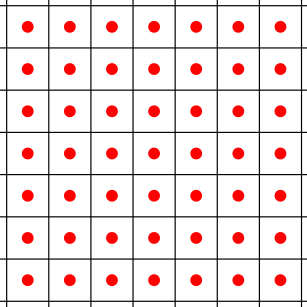
\includegraphics[width=0.6\textwidth]{resize1.png}\\

We consider the intensity of a pixel to be in its center.
\end{frame}


\begin{frame}
\frametitle{Informácia v obraze}
\centering
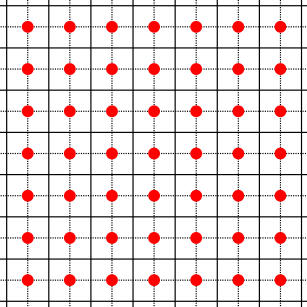
\includegraphics[width=0.6\textwidth]{resize2.png} \\

Dashed grid therefore shows the centers of pixels not their boundaries.
\end{frame}

\begin{frame}
\frametitle{Information in images}
\centering

\includegraphics[width=0.6\textwidth]{resize3.png}
\end{frame}


\begin{frame}
\frametitle{Resizing - Enlargement}
\centering
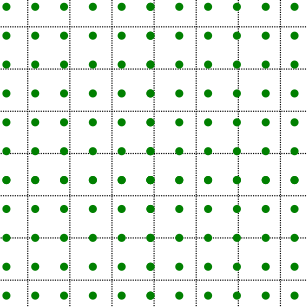
\includegraphics[width=0.6\textwidth]{resize4.png}
\end{frame}


\begin{frame}
\centering
\frametitle{Resizing - Reduction}
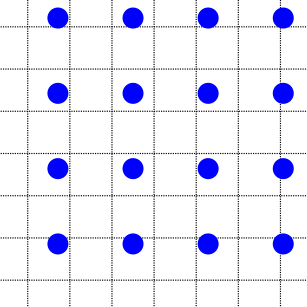
\includegraphics[width=0.6\textwidth]{resize5.png}
\end{frame}

\begin{frame}
\centering
\frametitle{Interpolácia}
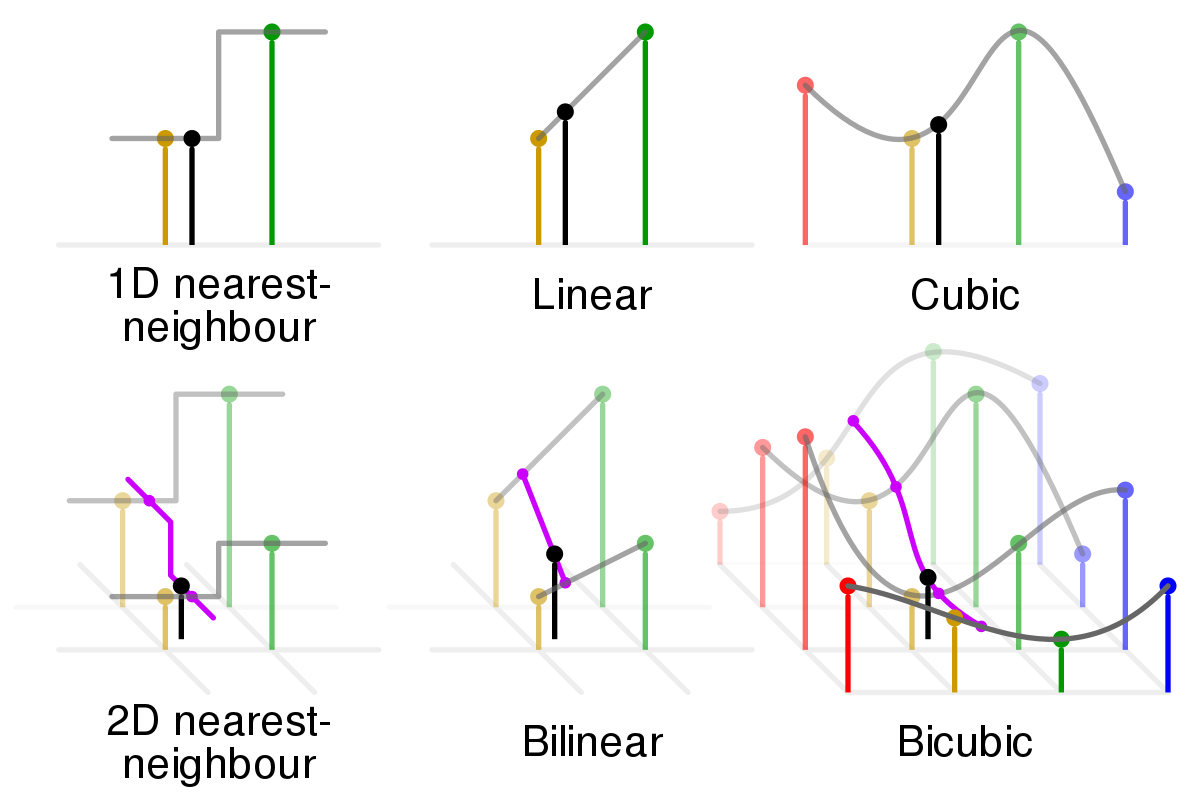
\includegraphics[width=0.8\textwidth]{interpolation.png} \\
How the value of the new pixel is calculated is given by interpolation.
\end{frame}


\begin{frame}
\centering
\frametitle{Resizing in Matlab}
\begin{block}{imresize}
imresize(I, scale) - returns the image I resized by the scale factor
\end{block}

\begin{block}{imresize}
imresize(I, [r, c]) - returns the image I resized to size $r \times c$
\end{block}

\begin{block}{imresize}
imresize(I, s, 'method') - returns the resized image I with the use of method: 'nearest', 'bilinear', 'bicubic'.
\end{block}

\begin{block}{Exercise}
Test resizing with different methods for the image shell.jpg and zatisie.jpg
\end{block}
\end{frame}

\section{Image Transformation}

\begin{frame}
\centering
\frametitle{Affine transformation}
\begin{block}{How is it calculated}
The transform is given by the following equation where $\vec{y}$ is the new position of the pixel.
$$ \vec{y} = \mathbb{A}\vec{x} + \vec{t}$$
\end{block}

\begin{alertblock}{Calculation for images}
When considering images we do not calculate $\vec{y}$ based on pixel positions $\vec{x}$, but instead we first choose some regular grid of $\vec{y}$ vectors and then calculate their respective position in the image using the inverse transform $\vec{x} = \mathbb{A}^{-1} (\vec{y} -\vec{t})$. This allows us to use interpolation in a straightforward fashion.
\end{alertblock}
\end{frame}

\begin{frame}
\centering
\frametitle{Exercises}
\begin{block}{Rotation}
$$ \mathbb{A} = \begin{bmatrix}
    cos(\alpha)       & -sin(\alpha)  \\
    sin(\alpha)       & cos(\alpha)  \\   
\end{bmatrix}$$
\end{block}

\begin{block}{x-axis scaling}
$$ \mathbb{A} = \begin{bmatrix}
    2       & 0  \\
    0       & 1  \\   
\end{bmatrix}$$
\end{block}
\end{frame}

\begin{frame}
\centering
\frametitle{Rotation}

\includegraphics[width=0.6\textwidth]{rotate.png}
\end{frame}

\begin{frame}
\centering
\frametitle{Affine transform}

\includegraphics[width=0.6\textwidth]{afine.png}
\end{frame}


\begin{frame}
\frametitle{Affine transformation in Matlab}
\begin{block}{imtransform}
imtransform(I, tform, interp) - transforms the image I with a transformation object t from using interpolation method interp: 'nearest', 'bilinear', 'bicubic'.
\end{block}

\begin{block}{maketform}
maketform('affine', B) - retursn transformation object for affine transformation. The transformation is defined with matrix B, which in our definition is the matrix A with additional column containing the vector $\vec{t}$.
\end{block}

\begin{block}{imrotate}
imrotate(I, angle) - returns the image I rotated by the given angle.
\end{block}
\end{frame}


\begin{frame}
\frametitle{Exercises}
\begin{block}{Exercises}
Perform a rotation of an image using imrotate. Try to accomplish the same result with affine transformation.
\end{block}

\begin{block}{Exercise}
Construct and affine transformation which flips just the x or y axis.
\end{block}

\begin{block}{Exercise}
Test various matrices for affine transformation.
\end{block}
\end{frame}


\begin{frame}
\frametitle{Perspective transformation}
\begin{block}{imtransform}
imtransform(I, tform, interp) - transforms the image I with a transformation object t from using interpolation method interp: 'nearest', 'bilinear', 'bicubic'.
\end{block}

\begin{block}{maketform}
maketform('projective', U, X) - returns a transformation object for perspective transformation. The matrices U and X are of shape $4 \times 2$. Each row of U is transformed to the corresponding row in X.
\end{block}

\begin{block}{Matrices U and X}
We can create the U matrix by calling U = ginput(4). We can use ginput to create X as well, or in case of rectification (making an object axis aligned) we can create a matrix in which each row is a different corner of a rectangle.
\end{block}
\end{frame}


\begin{frame}
\frametitle{Exercises}
\begin{block}{Exercise}
In the image qr.jpg use the perspective transformation in a way so that the QR code is rectified. Perform the same with the image book.jpg.
\end{block}

\begin{block}{Exercise}
In the image road.png use the perspective transformation so that the traffic lines are aligned with the y-axis. Is this task well-defined?
\end{block}
\end{frame}




\end{document}